\documentclass{iansnotes}

\title{Electrons and Photons}
\author{ian.mcloughlin@atu.ie}
\date{Last updated: \today}

\begin{document}
 
\maketitle

\section{Dividing Gold}

\begin{figure}
\begin{tikzpicture}
  \node[inner sep=0pt] (f)  at (0, 0) {
\includegraphics[width=40mm]{img/goldbar.png}};
  \node[inner sep=0pt] (h1) at (6, 2) {
\includegraphics[width=20mm]{img/goldbar.png}};
  \node[inner sep=0pt] (h2) at (6,-2) {
\includegraphics[width=20mm]{img/goldbar.png}};
  \node[inner sep=0pt] (q1) at (10, 3) {
\includegraphics[width=10mm]{img/goldbar.png}};
  \node[inner sep=0pt] (q2) at (10, 1) {
\includegraphics[width=10mm]{img/goldbar.png}};
  \node[inner sep=0pt] (q3) at (10,-1) {
\includegraphics[width=10mm]{img/goldbar.png}};
  \node[inner sep=0pt] (q4) at (10,-3) {
\includegraphics[width=10mm]{img/goldbar.png}};
  
  \draw[->,thick]  (f.east) -- node[above] {$\frac{1}{2}$} (h1.west);
  \draw[->,thick]  (f.east) -- node[below] {$\frac{1}{2}$} (h2.west);
  \draw[->,thick] (h1.east) -- node[above] {$\frac{1}{4}$} (q1.west);
  \draw[->,thick] (h1.east) -- node[below] {$\frac{1}{4}$} (q2.west);
  \draw[->,thick] (h2.east) -- node[above] {$\frac{1}{4}$} (q3.west);
  \draw[->,thick] (h2.east) -- node[below] {$\frac{1}{4}$} (q4.west);
\end{tikzpicture}
\end{figure}

\section{Photoelectric Effect}

\begin{figure}
  \begin{circuitikz}[
    lightbulb/.style={draw=gray!50,decorate,decoration={expanding waves,angle=20}}
  ]
  \ctikzset{tubes/height=3,tubes/width=0.7}
  \draw (4,2) node[diodetube,rotate=-90] (vacc) {};
  \draw
    (0,0)
    to[battery,invert]
    (8,0)
    to[ammeter]
    (8,2)
    to[short]
    (vacc.anode)
    (vacc.cathode)
    to[short]
    (1,2)
    to[short]
    (0,2)
    to[short]
    (0,0);
  \draw[lightbulb] (5,3) node[circle,fill=violet,draw=gray!50] {}  -- (vacc.tube bottom center);
  \end{circuitikz}
\end{figure}
\marginnote{\bibentry{photoelectriceffectbritannica}}

\begin{figure}
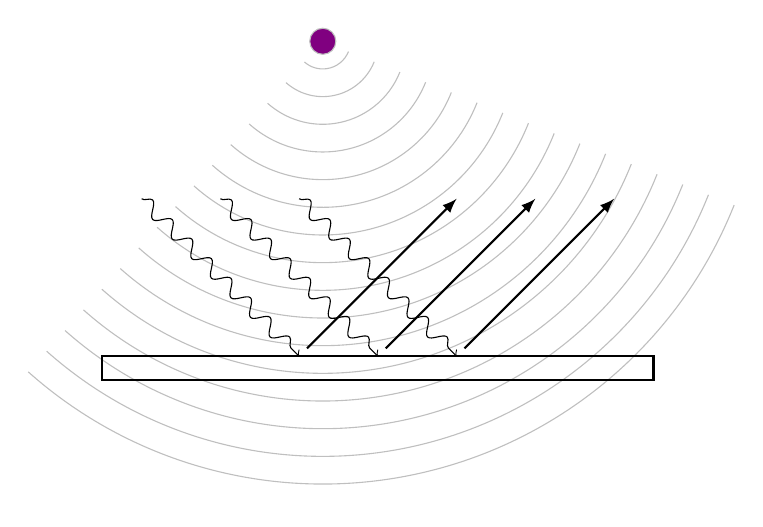
\begin{tikzpicture}[
  photon/.style={->,decorate,decoration={snake,post length=1mm}},
  electron/.style={-latex,thick},
  lightbulb/.style={draw=gray!50,decorate,decoration={expanding waves,angle=55}}
]
  \draw[lightbulb] (0.3,0) node[circle,fill=violet,draw=gray!50] {}  -- (1.6,-5.5);
  \draw[thick] (-2.5,-4) rectangle ++(7,-0.3) ;

  \begin{scope}[shift={(-2,-4)}]
    \draw[photon]   (0,2) -- (2,0);
    \draw[electron] (2.1,0.1) -- (4,2);
    \draw[photon]   (1,2) -- (3,0);
    \draw[electron] (3.1,0.1) -- (5,2);
    \draw[photon]   (2,2) -- (4,0);
    \draw[electron] (4.1,0.1) -- (6,2);
  \end{scope}
\end{tikzpicture}
\end{figure}

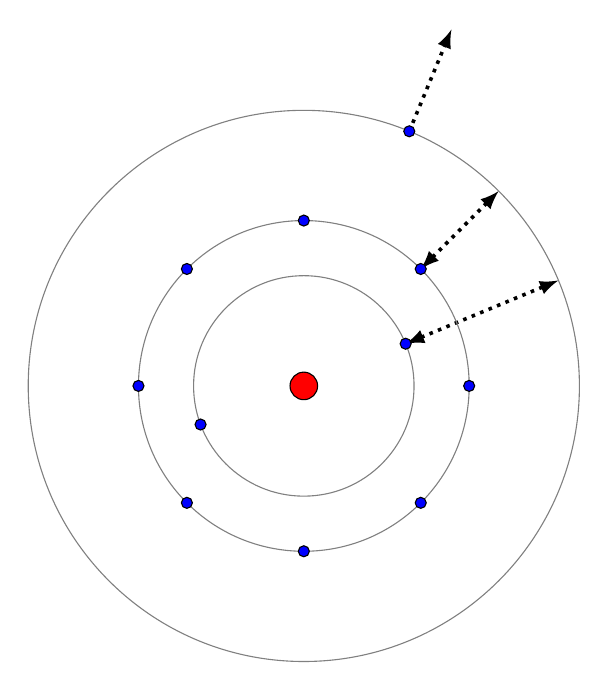
\begin{tikzpicture}[scale=0.7,
  transition/.style={latex-latex,line width=1.3pt,dotted,draw=black},
  orbit/.style={draw=gray},
  electron/.style={fill=blue},
  nucleus/.style={fill=red}
]
  \draw[transition] (45:3) -- (45: 5);
  \draw[transition] (22.5:2) -- (22.5: 5);
  \draw[transition,-latex] (67.5:5) -- (67.5:7);
  \draw[nucleus] (0,0) circle (0.25);
  \draw[orbit] (0,0) circle (2);
  \draw[orbit] (0,0) circle (3);
  \draw[orbit] (0,0) circle (5);
  \foreach \e in {22.5,200.5}
    \draw[electron] (\e:2) circle (0.1);
  \foreach \e in {0,45,90,...,315}
    \draw[electron] (\e:3) circle (0.1);
  \draw[electron] (67.5:5) circle (0.1);
\end{tikzpicture}

\end{document}